\chapter{Cadenas de Markov ocultas infinitas} 
\label{sec:proyecto}

En el capítulo anterior se introdujo el modelo de cadenas de Markov ocultas como una formulación probabilística para describir la coexistencia de un proceso latente y una secuencia observable. En el contexto musical, esta idea permitió interpretar las notas observadas como emisiones generadas por un mecanismo interno no directamente visible, el cual puede asociarse a una estructura armónica, a una región tonal o, más generalmente, a un contexto musical subyacente.

Tal descripción resulta adecuada siempre que se acepte que la dinámica latente puede resumirse en un conjunto finito de estados. El problema de este capítulo aparece precisamente cuando esa hipótesis comienza a quedarse corta para describir un vocabulario armónico más flexible.

Así, el cambio respecto del capítulo anterior no consiste en introducir un objeto musical distinto, sino en reformular una decisión de modelado que hasta ahora permanecía fija. En el HMM finito, una vez elegido el número de estados, los algoritmos de evaluación e inferencia pueden aplicarse de manera directa; pero en aplicaciones musicales esa elección rara vez es inocua. Un vocabulario demasiado pequeño fusiona contextos armónicos con funciones distintas, mientras que uno demasiado grande fragmenta regularidades que sería preferible mantener unificadas.

La pregunta guía del capítulo puede formularse así: si la idea latente-observable del HMM sigue siendo musicalmente útil, pero el número de estados deja de ser evidente, ¿cómo permitir que el propio modelo ajuste su complejidad al repertorio analizado? Para responderla, primero se fija una línea base finita y después se introduce la extensión no paramétrica que relaja esa decisión.

En una formulación armónica concreta, el HMM clásico exige fijar primero un conjunto finito $S$ de acordes permitidos y, una vez enumerado, identificar el espacio de estados ocultos con
\[
\mathcal{S}=\{1,2,\dots,N\},
\qquad N=\lvert S\rvert.
\]
La elección de $S$ determina simultáneamente la dimensión de la distribución inicial $\boldsymbol{\pi}$, de la matriz de transición $\mathbf{A}$ y de la familia de distribuciones de emisión $\mathbf{B}$. Para mantener comparabilidad e interpretabilidad, se adopta un vocabulario armónico finito construido como pares de la forma
\[
(\text{fundamental},\text{plantilla armónica}).
\]
El primer componente recoge la clase de altura y el segundo la sonoridad admitida.

Sea
\[
\mathcal{R}
=
\{C,C^\sharp,D,E^\flat,E,F,F^\sharp,G,A^\flat,A,B^\flat,B\}
\]
el conjunto de clases de altura fundamentales. Sea además
\[
\mathcal{Q}=
\left\{
\begin{array}{@{}l@{}}
\mathrm{Maj},\mathrm{min},\mathrm{dim},\mathrm{aug},\\
\mathrm{Maj7},7,\mathrm{m7},\mathrm{m(Maj7)},\varnothing 7,\mathrm{dim7},\\
6,\mathrm{m6},\mathrm{add9},\mathrm{madd9},6/9,\\
\mathrm{sus2},\mathrm{sus4},7\mathrm{sus4},\\
\mathrm{Maj9},9,\mathrm{m9}
\end{array}
\right\}
\]
la familia de plantillas armónicas admitidas. Con ello se obtiene un repertorio suficientemente rico para distinguir triadas, séptimas, suspensiones y extensiones frecuentes sin volver opaco el espacio latente.

Se define entonces
\[
S=\mathcal{R}\times\mathcal{Q}.
\]
En consecuencia,
\[
\lvert S\rvert = 12\times 21 = 252.
\]
Este tamaño sigue siendo manejable para un HMM finito con observaciones discretas y evita colapsar sonoridades distintas sobre una misma triada elemental. Sin embargo, la decisión sigue siendo exógena: si $N$ es demasiado pequeño, el modelo fusiona funciones distintas; si es demasiado grande, fragmenta regularidades y dispersa masa de probabilidad. El problema central, entonces, no es sólo enriquecer el vocabulario armónico, sino permitir que la complejidad efectiva del espacio latente dependa de los datos y no de una elección previa.

\section{Modelos bayesianos no paramétricos para secuencias musicales}

La situación anterior conduce al marco de los modelos bayesianos no paramétricos. Aquí \emph{no paramétrico} no significa ausencia de parámetros, sino ausencia de una cota fijada de antemano para la complejidad estructural del modelo. La herramienta central es el proceso de Dirichlet, que permite definir distribuciones a priori sobre medidas de probabilidad discretas \cite{ferguson1973,sethuraman1994}. Una discusión más amplia de esta construcción y de su versión jerárquica se deja al Apéndice A; en el cuerpo principal basta retener que el objetivo es reemplazar la elección exógena de $N$ por un mecanismo probabilístico capaz de reutilizar estados ya activados y, al mismo tiempo, introducir nuevos cuando la secuencia lo exige.

La primera extensión natural del HMM clásico consiste entonces en reemplazar el espacio finito de estados ocultos por un conjunto numerable infinito, que para fijar ideas se identifica con
\[
\mathcal{S}=\mathbb{N}.
\]
La hipótesis markoviana no se modifica: el futuro del proceso oculto depende únicamente del estado oculto presente, y cada observación depende solamente del estado latente actual. Lo que cambia es la cardinalidad del conjunto sobre el cual se definen las transiciones.

\begin{Definicion}
Una \emph{cadena de Markov oculta infinita} está determinada por dos procesos estocásticos en tiempo discreto
\[
(X_n)_{n\geq 0}, \qquad (Y_n)_{n\geq 0},
\]
donde $(X_n)$ toma valores en $\mathbb{N}$ y $(Y_n)$ toma valores en un espacio de observaciones $\mathcal{V}$. Se fija una distribución inicial
\[
\boldsymbol{\pi}=(\pi_i)_{i\geq 1},
\]
una matriz de transición infinita
\[
\mathbf{A}=(a_{ij})_{i,j\geq 1},
\]
y una familia de distribuciones de emisión
\[
\mathbf{B}=(b_j)_{j\geq 1},
\]
de modo que, para todo $i,j\geq 1$ y todo $v\in\mathcal{V}$,
\[
P(X_0=i\mid \boldsymbol{\pi})=\pi_i,
\]
\[
P(X_{n+1}=j\mid X_n=i,\mathbf{A})=a_{ij},
\qquad
P(Y_n=v\mid X_n=j,\mathbf{B})=b_j(v),
\]
con
\[
\sum_{i=1}^{\infty}\pi_i=1,
\qquad
\sum_{j=1}^{\infty}a_{ij}=1,
\qquad
\sum_{v\in\mathcal{V}}b_j(v)=1.
\]
\end{Definicion}

La definición anterior extiende literalmente la formulación del HMM al caso de un espacio de estados ocultos numerable. La estructura markoviana y la factorización de la ley conjunta se conservan; lo que cambia es la forma de controlar la complejidad del espacio latente.

La dificultad principal consiste en coordinar coherentemente los renglones de una matriz de transición infinita. Para ello se introduce una medida global que actúa como soporte compartido de las distribuciones de transición. Esta construcción conduce al proceso de Dirichlet jerárquico y, en el contexto de cadenas de Markov ocultas, al \emph{HDP-HMM} (\emph{Hierarchical Dirichlet Process Hidden Markov Model}), que proporciona una realización concreta del \emph{Infinite Hidden Markov Model (iHMM)} \cite{beal2002,teh2006}.

En esta formulación se introduce una medida discreta aleatoria global
\[
\beta=\sum_{k=1}^{\infty}\beta_k\delta_k,
\]
donde
\[
\beta_k=v_k\prod_{\ell=1}^{k-1}(1-v_{\ell}),
\qquad
v_k \overset{i.i.d.}{\sim}\mathrm{Beta}(1,\gamma),
\qquad k\geq 1,
\]
y se supone que
\[
\boldsymbol{\pi}\mid \beta \sim DP(\alpha_0,\beta),
\qquad
A_i\mid \beta \sim DP(\alpha,\beta), \qquad i\geq 1,
\]
donde $A_i$ denota el renglón $i$-ésimo de $\mathbf{A}$.
\[
\mathbb{E}[a_{ij}\mid\beta]=\beta_j.
\]
La medida global $\beta$ asigna pesos a una familia numerable de estados potenciales y acopla todas las distribuciones de transición al imponerles un soporte común. En términos musicales, esto permite reutilizar contextos latentes ya presentes sin impedir que aparezcan otros cuando la evidencia secuencial lo justifica.

Cuando el espacio observable $\mathcal{V}$ es finito, como ocurre al modelar notas, clases de altura, intervalos o símbolos rítmicos discretizados, la familia de emisiones $\mathbf{B}$ puede mantenerse dentro de una parametrización finita ordinaria. En muchas aplicaciones musicales esta decisión es suficiente, porque la principal fuente de incertidumbre no suele residir en el alfabeto observable, sino en cuántos contextos latentes hacen falta para organizarlo en el tiempo.

La infinitud del espacio de estados no implica que una pieza finita requiera infinitos contextos latentes, sino que el modelo deja abierta esa complejidad y la delega a la inferencia. Ésta es la diferencia decisiva frente al HMM clásico: en lugar de fijar primero el número de estados y luego estimar transiciones y emisiones, el iHMM permite que la estructura latente emerja del comportamiento observado. Para el análisis musical, esto significa que distinciones armónicas, melódicas o formales sólo se separan cuando los datos ofrecen evidencia suficiente para hacerlo.



\section{Aproximación truncada y formulación computacional}

La formulación infinita descrita en la sección anterior tiene valor conceptual, pero su uso directo en inferencia complica la implementación porque la programación dinámica debe operar sobre un conjunto no acotado de estados potenciales. Por ello, en la práctica se emplea una aproximación truncada que conserva la estructura jerárquica del HDP-HMM y la proyecta sobre un simplex finito de dimensión $K$ \cite{ishwaran2001,fox2011,vangael2008}.

\begin{Definicion}
Fijado un entero $K\geq 2$, un \emph{HDP-HMM truncado} con espacio observable discreto $\mathcal{V}=\{1,\dots,V\}$ queda determinado por las variables aleatorias
\[
v_k\sim \mathrm{Beta}(1,\gamma), \qquad k=1,\dots,K-1,
\]
\[
\beta_k=v_k\prod_{\ell=1}^{k-1}(1-v_{\ell}), \qquad k=1,\dots,K-1,
\]
\[
\beta_K=\prod_{\ell=1}^{K-1}(1-v_{\ell}),
\]
por el vector global $\beta=(\beta_1,\dots,\beta_K)$ y por las distribuciones condicionadas
\[
\boldsymbol{\pi}\mid \beta \sim \mathrm{Dir}(\alpha_0\beta_1,\dots,\alpha_0\beta_K),
\]
\[
A_i\mid \beta \sim \mathrm{Dir}(\alpha\beta+\kappa e_i), \qquad i=1,\dots,K,
\]
\[
\phi_i\sim \mathrm{Dir}\left(\frac{\eta}{V},\dots,\frac{\eta}{V}\right), \qquad i=1,\dots,K,
\]
donde $e_i$ denota el $i$-ésimo vector canónico de $\mathbb{R}^K$. La cadena latente y las observaciones satisfacen entonces
\[
X_1\mid \boldsymbol{\pi}\sim \mathrm{Cat}(\boldsymbol{\pi}),
\qquad
X_t\mid X_{t-1}=i,\mathbf{A}\sim \mathrm{Cat}(A_i),
\]
\[
Y_t\mid X_t=i,\phi_i\sim \mathrm{Cat}(\phi_i), \qquad t\geq 1.
\]
\end{Definicion}

La escritura anterior conserva la lógica del modelo infinito: $\beta$ organiza el soporte compartido, $\alpha_0$ regula la distribución inicial y $\alpha$ controla cuánto puede apartarse cada renglón de la estructura global. En la práctica, lo importante es escoger un $K$ suficientemente amplio para que funcione como cota técnica y no como restricción activa. Una vez fijado, las transiciones y emisiones pueden manejarse como matrices finitas y la trayectoria latente puede inferirse con programación dinámica estándar, con costo dominante del orden de $O(TK^2)$.

En esta tesis, el modelo truncado se especializa al caso de observaciones categóricas de clase de altura. El iHMM conserva así su papel como referencia conceptual, mientras que el HDP-HMM truncado se vuelve la realización operativa con la que se efectúan los experimentos reproducibles y la comparación con el HMM finito.

\section{De una obra al corpus}

Antes de pasar a resúmenes agregados conviene fijar un caso singular que obligue al modelo a mostrar su conducta en condiciones exigentes. En lugar de empezar por promedios, se toma como obra ancla el tercer movimiento de la Sonata no.\ 14 de Beethoven, una pieza extensa dentro del corpus extendido, con $4133$ notas y $201$ compases. La elección no pretende canonizar una sola obra, sino introducir una situación en la que el HMM finito tiende a fragmentar en exceso el espacio latente y donde, por tanto, la promesa del modelo no paramétrico puede evaluarse de forma visible.

La Tabla~\ref{tab:single-anchor} resume el contraste cuantitativo. El HMM finito activa $88$ estados, mientras que el HDP-HMM truncado concentra la trayectoria en $9$ estados efectivos y mejora la log-verosimilitud en $2408.011$ unidades. En esta escala, la diferencia relevante no es sólo estadística: también cambia el tipo de organización que el modelo atribuye a la pieza.

\begin{table}[H]
\centering
\small
\setlength{\tabcolsep}{4pt}
\begin{tabular}{@{}lrrrr@{}}
\hline
Modelo & $\log L$ & Estados & Segmentos & Long.\ media \\
\hline
HMM finito & -10242.186 & 88 & 560 & 7.380 \\
HDP-HMM truncado & -7834.175 & 9 & 1075 & 3.845 \\
\hline
\end{tabular}

\caption{Comparación entre el HMM finito y el HDP-HMM truncado sobre la obra ancla: el tercer movimiento de la Sonata no.\ 14 de Beethoven.}
\label{tab:single-anchor}
\end{table}

La Figura~\ref{fig:single-anchor-graph} permite leer esa diferencia de manera más directa. El panel izquierdo no representa toda la maraña del HMM finito, sino sus estados más ocupados; aun con esa poda, la estructura aparece dispersa y obliga a dejar fuera decenas de estados residuales. El panel derecho muestra el resultado contrario: el HDP-HMM truncado reutiliza un conjunto pequeño de contextos y conserva conexiones claras entre ellos. La reducción de complejidad no debe entenderse como empobrecimiento, sino como una compresión de redundancias que vuelve más legible la organización latente de una obra larga y densa.

\begin{figure}[H]
\centering
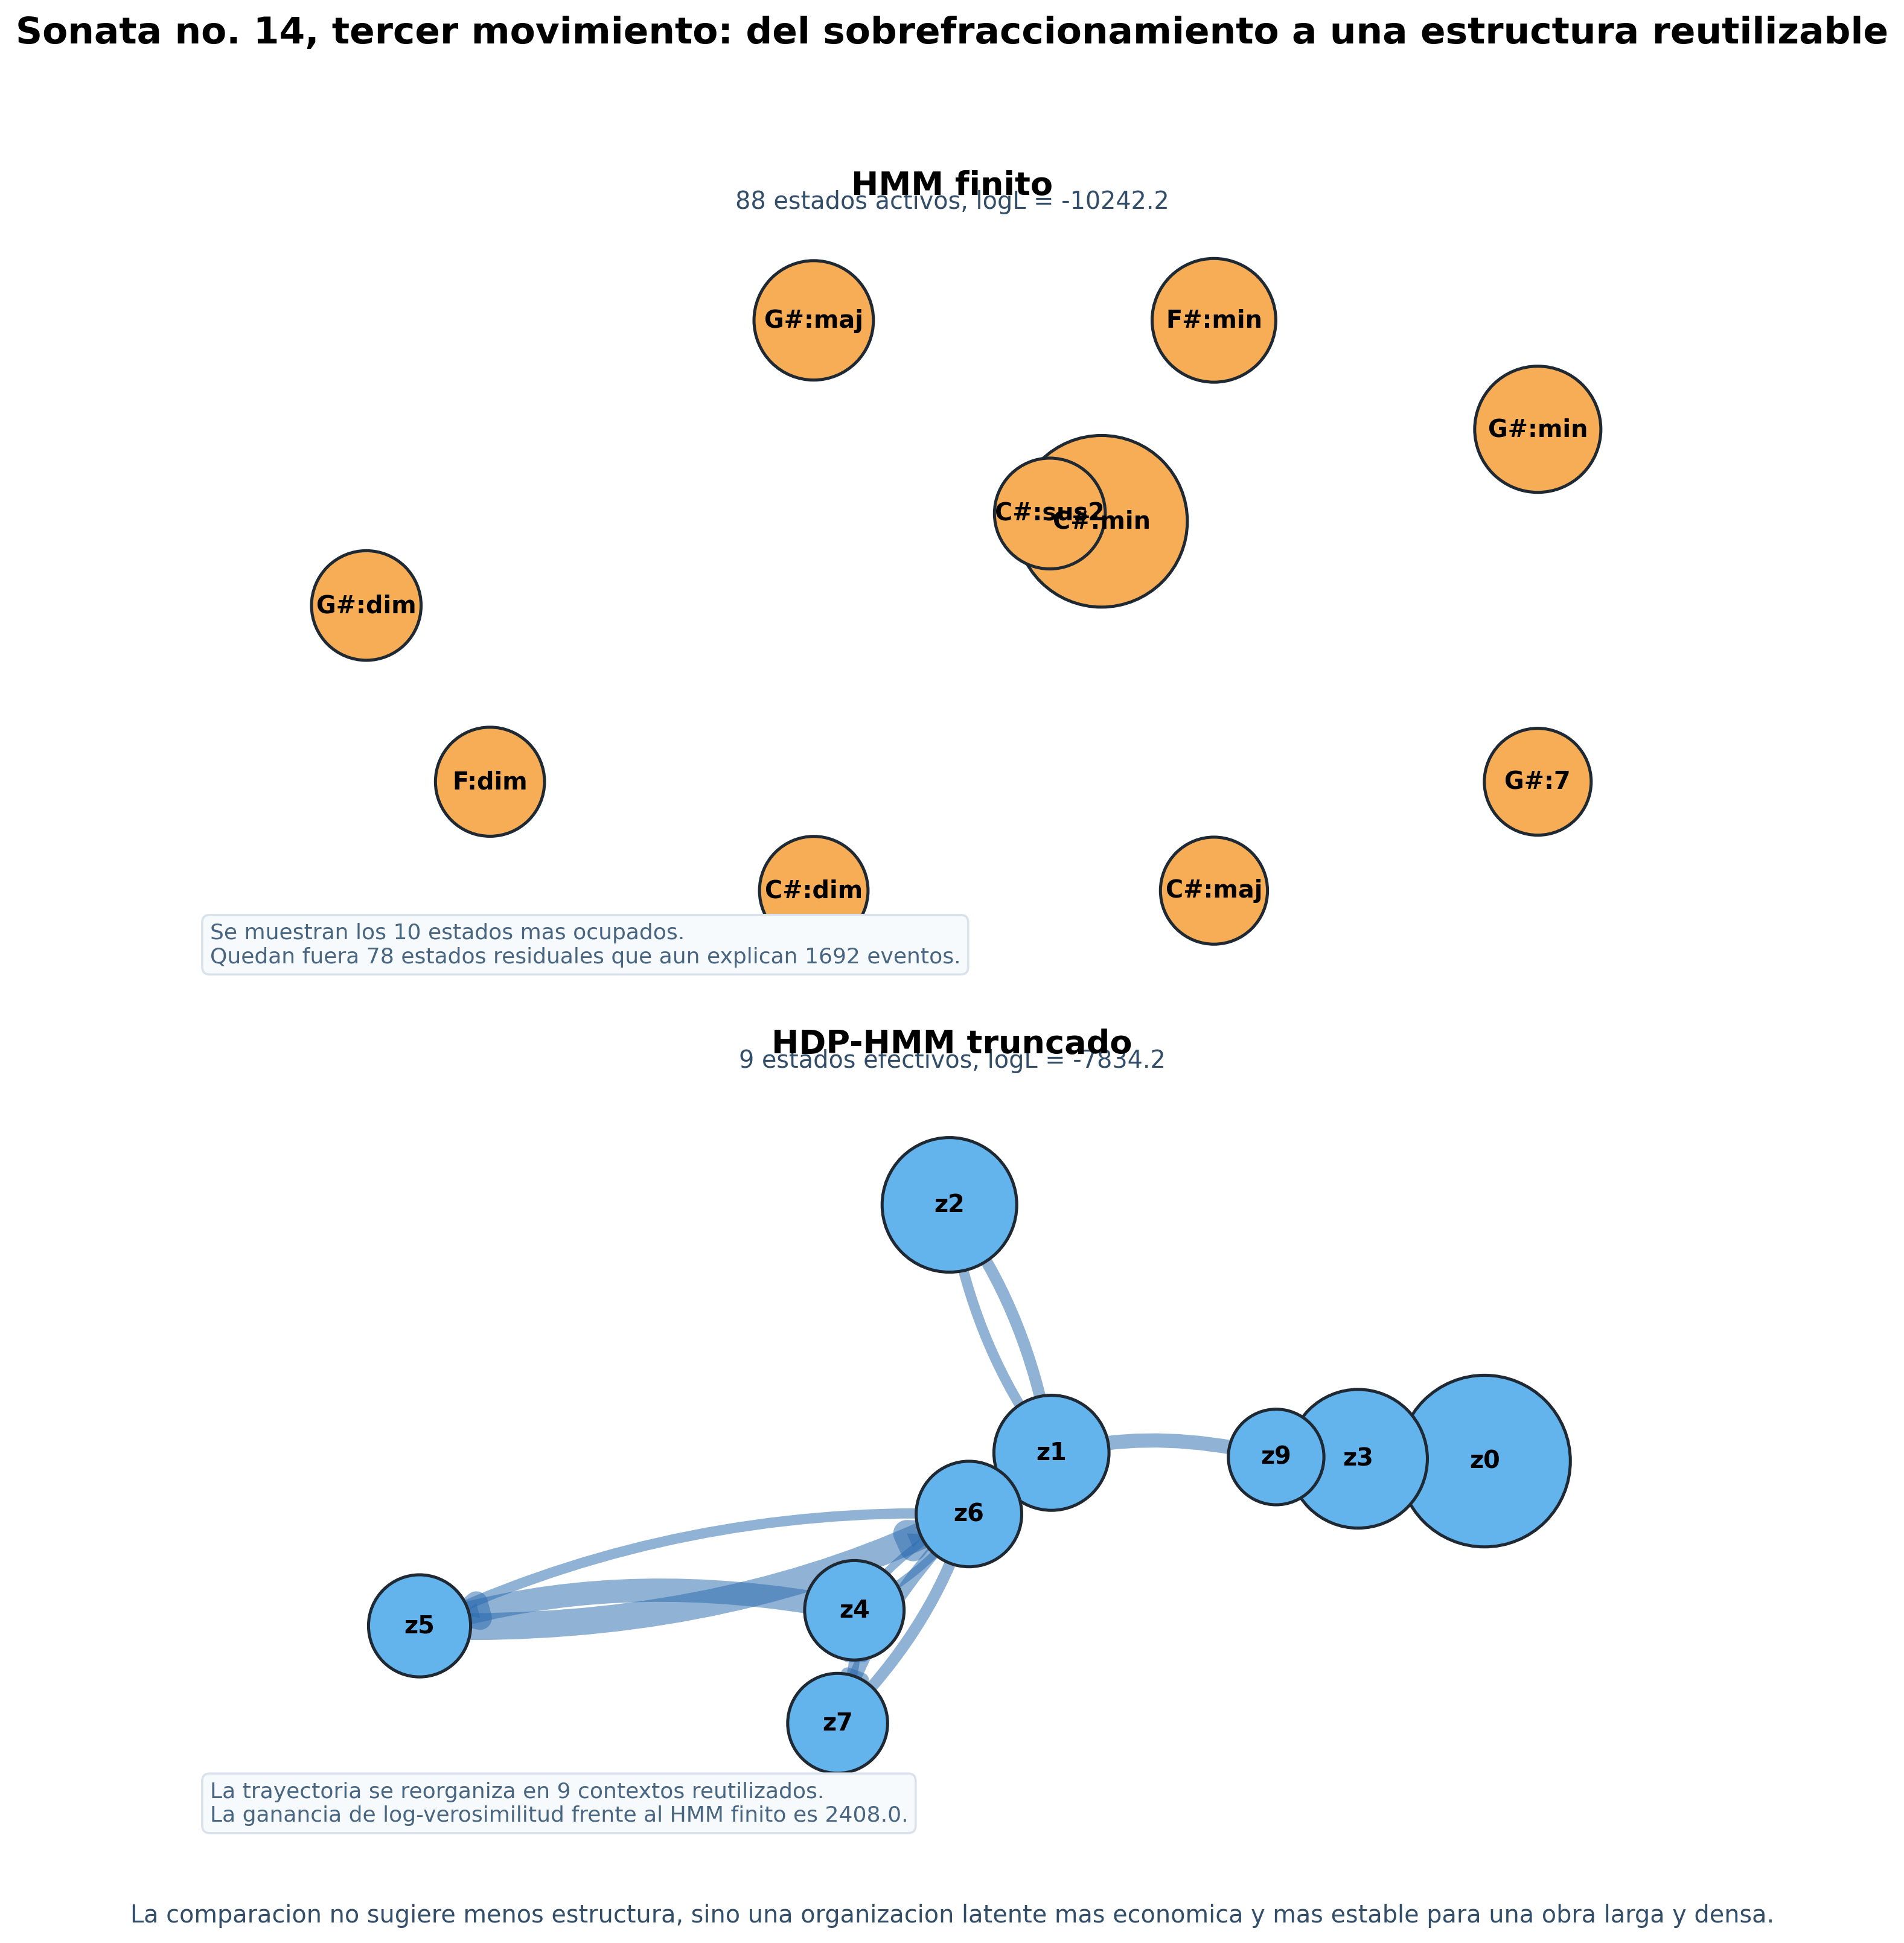
\includegraphics[width=\textwidth]{figures/chapter3/single_anchor_transition_comparison.png}
\caption{Obra ancla del capítulo. El HMM finito sobrefragmenta la trayectoria en una nube de estados activos, mientras que el HDP-HMM truncado reorganiza la misma secuencia en un conjunto mucho más compacto de contextos reutilizados.}
\label{fig:single-anchor-graph}
\end{figure}

Introducido el caso singular, el argumento necesita un control intermedio antes de generalizar al multicorpus. Por ello se conserva el caso base del capítulo como una escala reproducible de comparación: primero una obra difícil, después un subconjunto clásico pequeño y, sólo al final, el corpus heterogéneo de mayor tamaño.

\subsection{Resultados sobre un subconjunto clásico}

La evaluación comparativa se realizó sobre un subconjunto clásico limitado para mantener control experimental. La observación utilizada fue la clase de altura y el modelo truncado se ajustó con $K=12$, $\alpha=8$, $\alpha_0=4$, $\gamma=2$, $\eta=1$, $\kappa=0$, veinte iteraciones totales, diez de \emph{burn-in} y semilla igual a $7$. La Tabla~\ref{tab:corpus-clasico-limitado} resume las seis piezas breves utilizadas como base reproducible de comparación.

\begin{table}[H]
\centering
\footnotesize
\setlength{\tabcolsep}{4pt}
\begin{tabular}{@{}p{5.5cm}p{2.8cm}rr@{}}
\hline
Obra & Compositor & Notas & Compases \\
\hline
Cumpleanos feliz (Do mayor) & Tradicional & 37 & 8 \\
Oda a la alegria (variacion facil) & Desconocido & 87 & 17 \\
Para Elisa (version facil) & Beethoven & 103 & 22 \\
Cumpleanos feliz (arreglo) & Manjuprasad & 106 & 19 \\
Para Elisa (piano para principiantes) & Beethoven & 149 & 23 \\
Greensleeves & Desconocido & 166 & 33 \\
\hline
\end{tabular}

\caption{Subconjunto clásico limitado utilizado para la comparación reproducible entre el HMM finito y el HDP-HMM truncado.}
\label{tab:corpus-clasico-limitado}
\end{table}

La Tabla~\ref{tab:resumen-resultados-clasicos} condensa el resultado central: en las seis obras, el modelo truncado obtiene una log-verosimilitud superior a la del HMM finito. La ganancia media es de $92.970$ unidades, la mediana de $98.739$ y el número medio de estados efectivos del HDP-HMM truncado es menor que el número medio de estados activos del baseline finito.

\begin{table}[H]
\centering
\small
\begin{tabular}{lr}
\hline
Metrica & Valor \\
\hline
Obras comparables & 6 \\
Casos en que el HDP-HMM truncado mejora & 6 \\
Casos en que el HDP-HMM truncado empeora & 0 \\
Empates & 0 \\
Ganancia media de log-verosimilitud & 92.970 \\
Ganancia mediana de log-verosimilitud & 98.739 \\
Media de log-verosimilitud del HMM finito & -267.685 \\
Media de log-verosimilitud del HDP-HMM truncado & -174.715 \\
Estados activos medios del HMM finito & 10.833 \\
Estados efectivos medios del HDP-HMM truncado & 6.667 \\
\hline
\end{tabular}

\caption{Resumen agregado de la comparación entre el HMM finito y el HDP-HMM truncado sobre el subconjunto clásico limitado.}
\label{tab:resumen-resultados-clasicos}
\end{table}

La evidencia por obra aparece en la Tabla~\ref{tab:resultados-por-obra}. Dado que este experimento intermedio fue diseñado como control reproducible y no como corpus amplio, la tabla contiene sólo seis piezas. La magnitud de la mejora varía, pero el patrón es uniforme: ninguna favorece al modelo finito. Incluso en este repertorio sencillo, permitir que el número efectivo de estados se ajuste a la obra produce una ventaja estadística tangible.

\begin{table}[H]
\centering
\footnotesize
\setlength{\tabcolsep}{4pt}
\begin{tabular}{@{}p{4.2cm}p{2.1cm}rrrr@{}}
\hline
Obra & Compositor & Notas & $\log L_{fin}$ & $\log L_{hdp}$ & $\Delta \log L$ \\
\hline
Cumpleaños feliz (Do mayor) & Tradicional & 37 & -91.575 & -63.314 & 28.261 \\
Oda a la alegría (variación fácil) & Desconocido & 87 & -215.515 & -121.835 & 93.680 \\
Para Elisa (versión fácil) & Beethoven & 103 & -255.714 & -158.149 & 97.565 \\
Cumpleaños feliz (arreglo) & Manjuprasad & 106 & -262.027 & -162.114 & 99.914 \\
Greensleeves & Desconocido & 166 & -411.682 & -308.600 & 103.083 \\
Para Elisa (piano para principiantes) & Beethoven & 149 & -369.596 & -234.276 & 135.321 \\
\hline
\end{tabular}

\caption{Comparación por obra en las seis piezas del subconjunto clásico. La ganancia se calcula como la diferencia \mbox{HDP-HMM truncado $-$ HMM finito}.}
\label{tab:resultados-por-obra}
\end{table}

La Figura~\ref{fig:logverosimilitud-clasica} confirma visualmente el mismo patrón: todas las obras quedan del lado favorable al HDP-HMM truncado y la distribución agregada de log-verosimilitud también se desplaza en su favor.

\begin{figure}[H]
\centering
\begin{subfigure}[t]{0.88\textwidth}
\centering
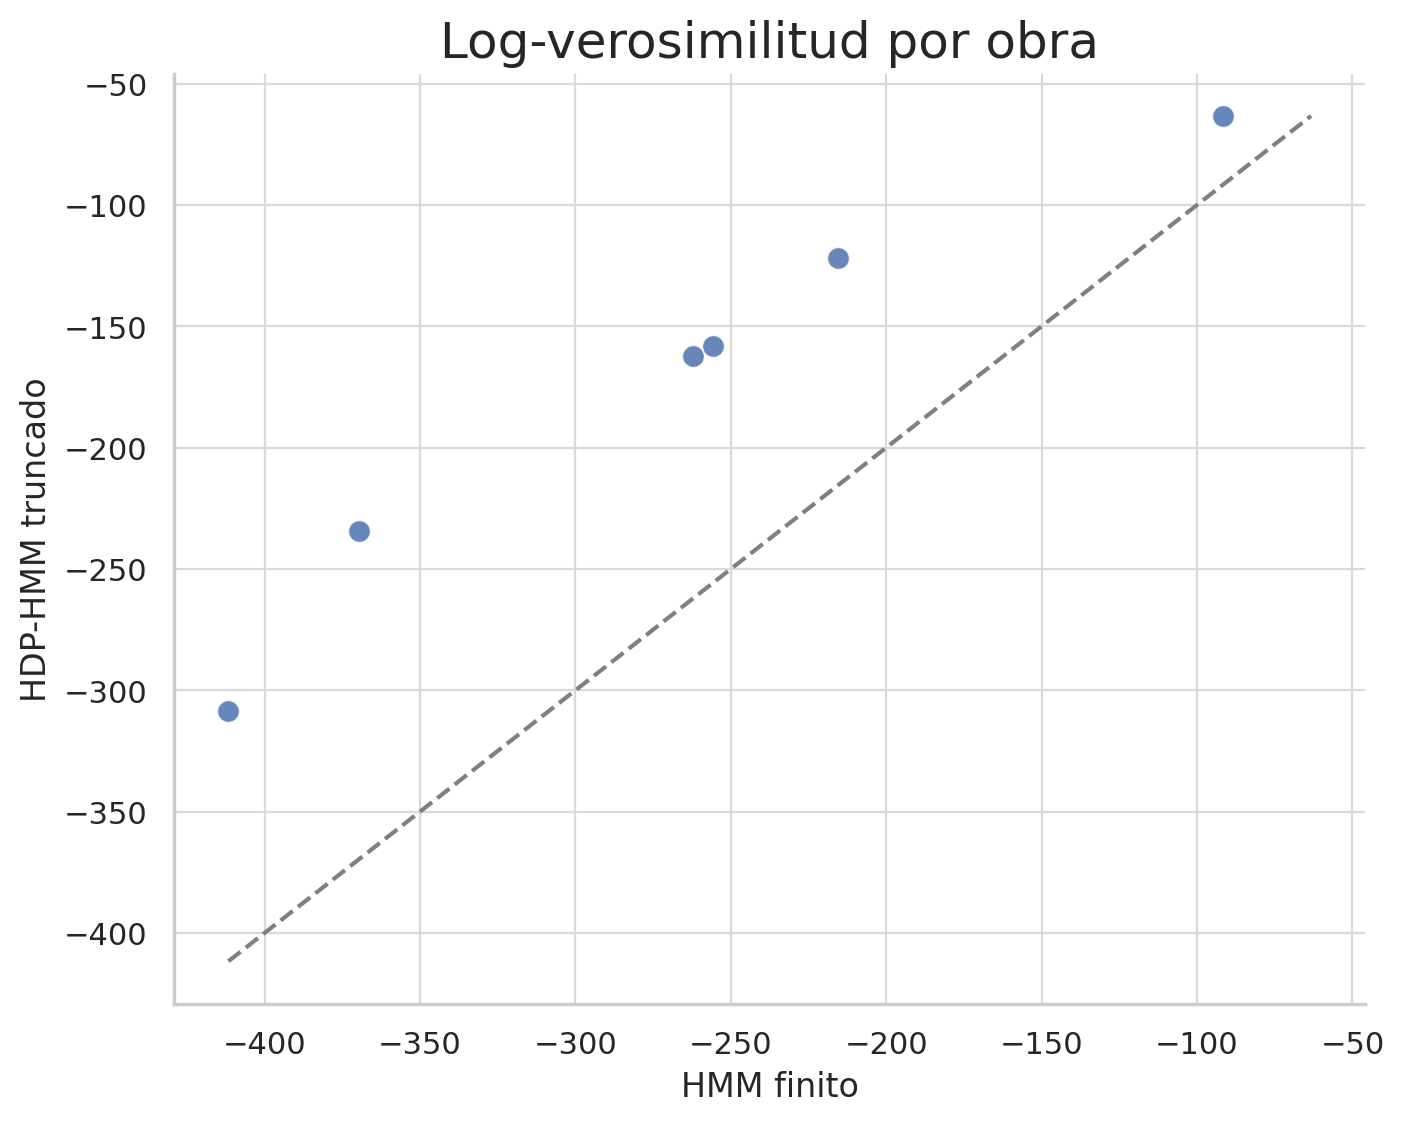
\includegraphics[width=\linewidth]{figures/chapter3/classic_log_likelihood_scatter.png}
\caption{Comparación de log-verosimilitud por obra.}
\end{subfigure}

\medskip
\begin{subfigure}[t]{0.88\textwidth}
\centering
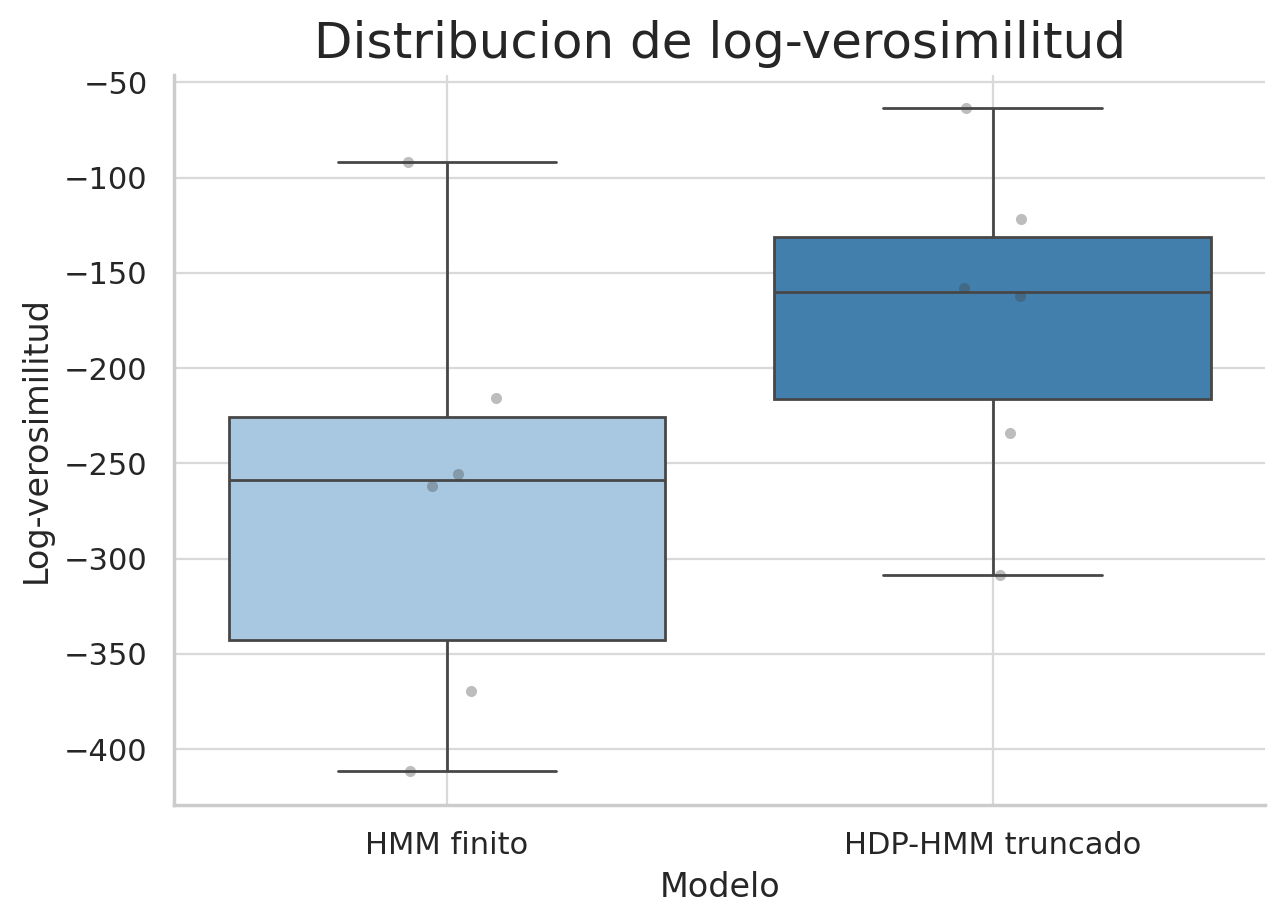
\includegraphics[width=\linewidth]{figures/chapter3/classic_log_likelihood_boxplot.png}
\caption{Distribución agregada de log-verosimilitud por modelo.}
\end{subfigure}
\caption{Lectura visual del ajuste probabilístico en el subconjunto clásico limitado. En ambos paneles, el desplazamiento favorece al HDP-HMM truncado.}
\label{fig:logverosimilitud-clasica}
\end{figure}

La Figura~\ref{fig:ganancia-y-complejidad-clasica} añade el segundo punto importante: la mejora no proviene de inflar indiscriminadamente la complejidad. El HDP-HMM truncado obtiene mejor ajuste y, al mismo tiempo, usa menos estados efectivos que el HMM finito.

\begin{figure}[H]
\centering
\begin{subfigure}[t]{0.88\textwidth}
\centering
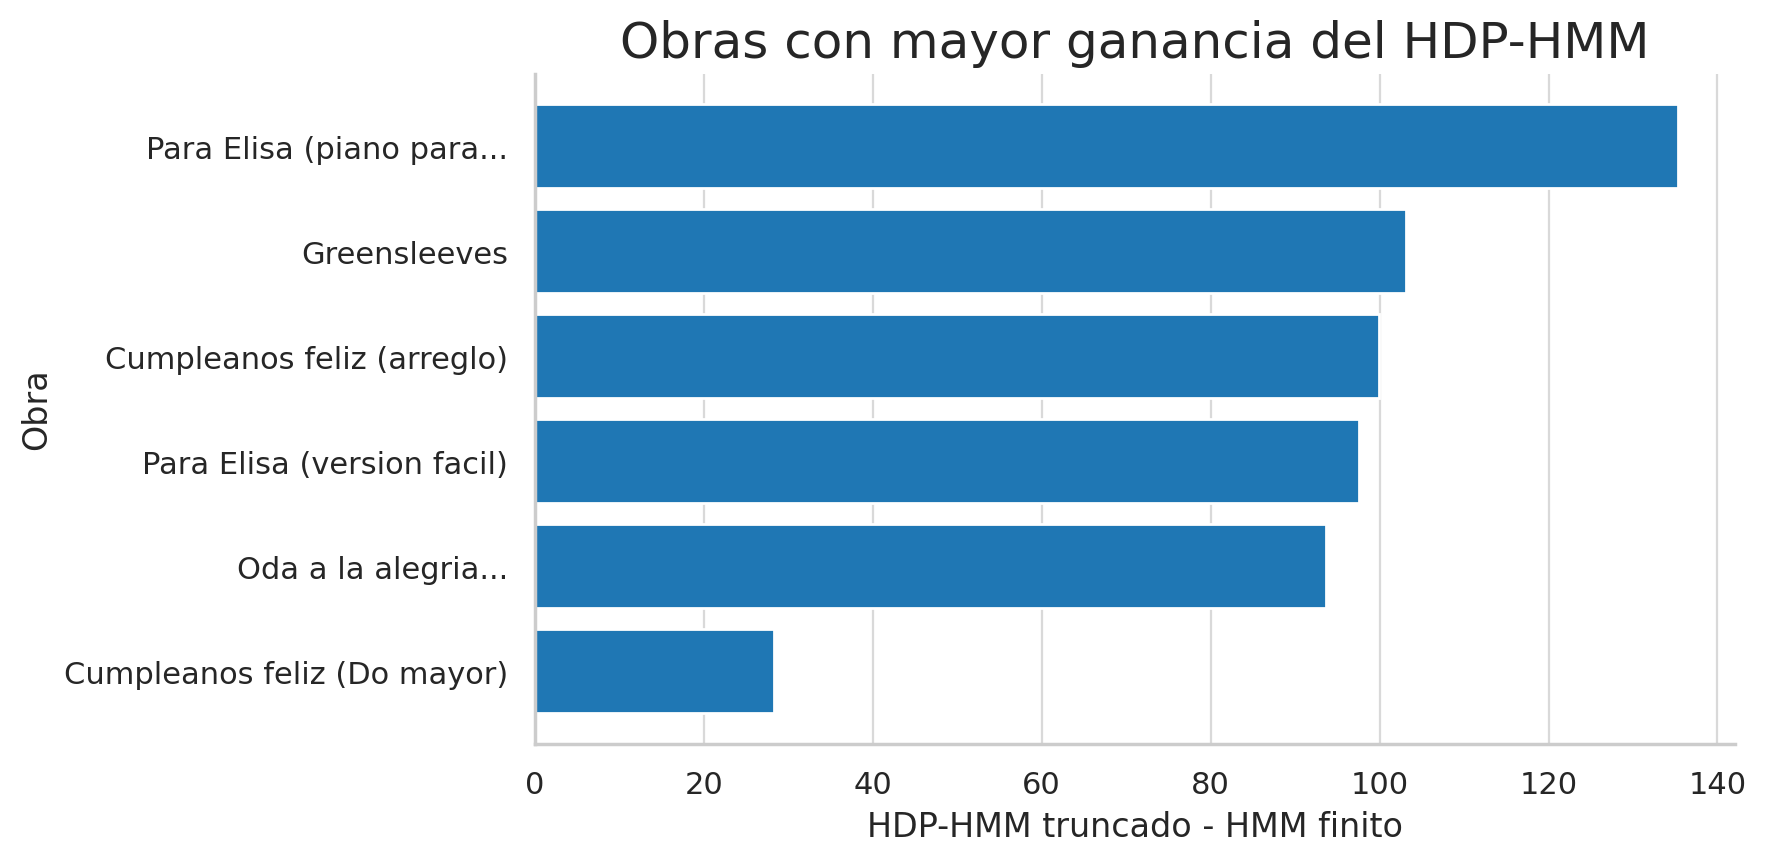
\includegraphics[width=\linewidth]{figures/chapter3/classic_log_likelihood_gain_by_piece.png}
\caption{Ganancia de log-verosimilitud por obra.}
\end{subfigure}

\medskip
\begin{subfigure}[t]{0.88\textwidth}
\centering
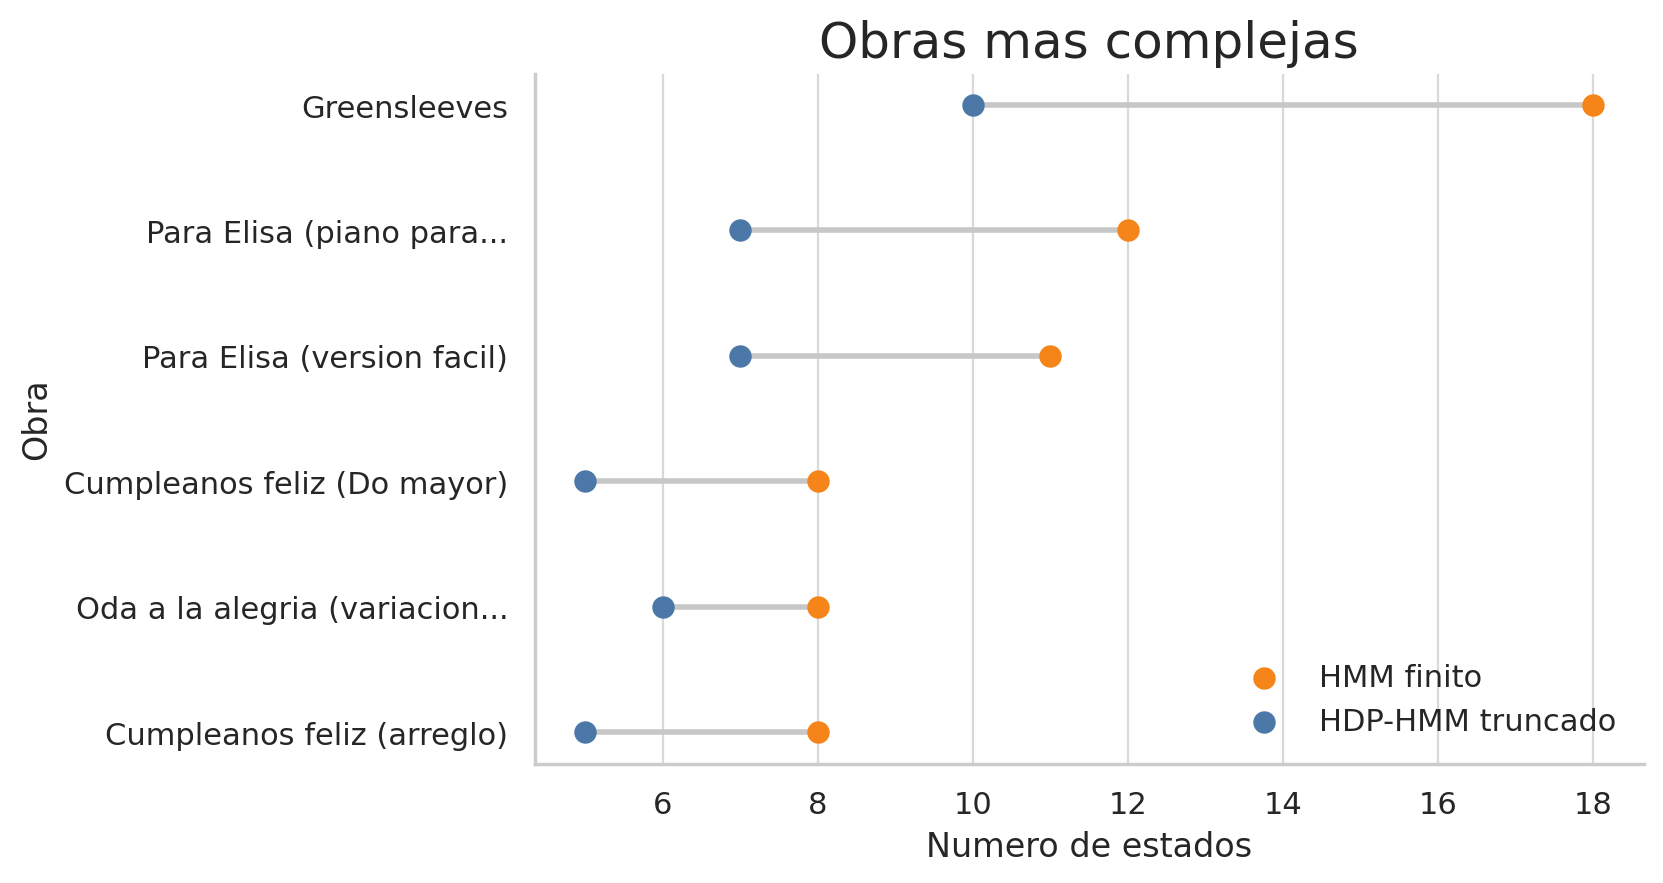
\includegraphics[width=\linewidth]{figures/chapter3/classic_state_counts_by_piece.png}
\caption{Comparación del número de estados por obra.}
\end{subfigure}
\caption{Descomposición visual de la ventaja del HDP-HMM truncado. El panel izquierdo mide la ganancia en ajuste y el derecho compara la complejidad latente efectiva de ambos modelos.}
\label{fig:ganancia-y-complejidad-clasica}
\end{figure}

Estos resultados deben leerse con cautela: el subconjunto es pequeño y la log-verosimilitud no agota la calidad musicológica de una segmentación latente. Su función dentro del capítulo es más específica: servir de puente entre la obra ancla y el multicorpus. Aun así, la evidencia basta para sostener la conclusión metodológica de esta sección: cuando no se fija \emph{ex ante} el número efectivo de estados, la aproximación truncada al iHMM mejora el ajuste y mantiene una complejidad posterior contenida.

\subsection{Resultados sobre el corpus extendido}

Una vez establecida la ventaja del modelo truncado en una obra exigente y en un subconjunto clásico controlado, conviene preguntar si esa ventaja se mantiene al ampliar el repertorio. Para ello se construyó un corpus extendido con dos fuentes: repertorio occidental etiquetado como \texttt{MuseTrainer} y material de tradición makam procedente de \texttt{SymbTr}. La Tabla~\ref{tab:corpus-extendido} resume su composición. El interés de esta ampliación no es homogeneizar ambos repertorios, sino probar la estabilidad del modelo cuando cambia de manera significativa el entorno estilístico.

\begin{table}[H]
\centering
\footnotesize
\setlength{\tabcolsep}{4pt}
\begin{tabular}{@{}p{2.2cm}p{8.2cm}r@{}}
\hline
Fuente & Perfil del material incorporado & Obras \\
\hline
MuseTrainer & Repertorio tonal occidental de orientacion pedagogica y clasica, con piezas breves y medianas en formato MusicXML. & 69 \\
SymbTr & Repertorio de musica artistica turca; el adaptador conserva metadatos de \emph{makam}, \emph{usul} y forma para preservar la procedencia modal. & 100 \\
\hline
Total & Corpus extendido usado para evaluar la estabilidad del modelo bajo mayor heterogeneidad estilistica. & 169 \\
\hline
\end{tabular}

\caption{Composición del corpus extendido utilizado en la comparación multicorpus.}
\label{tab:corpus-extendido}
\end{table}

De las $169$ obras catalogadas, $168$ pudieron correrse en la evaluación multicorpus y $167$ quedaron comparables entre ambos modelos; en la corrida base una obra de Mozart no entró al lote final y una pieza de Brahms arrojó un error de ejecución. Aun con esa salvedad, la evidencia es nítida. La Tabla~\ref{tab:resultados-multicorpus} muestra que el HDP-HMM truncado mejora la log-verosimilitud en las $167$ obras comparables. La ganancia media global asciende a $452.751$ unidades y la mediana a $377.039$, mientras que el número medio de estados efectivos del HDP-HMM truncado se mantiene cerca de $8$ frente a más de $32$ estados activos del HMM finito.

\begin{table}[H]
\centering
\footnotesize
\setlength{\tabcolsep}{4pt}
\begin{tabular}{lrrrrrrr}
\hline
Fuente & Obras & $\overline{\Delta \log L}$ & $\widetilde{\Delta \log L}$ & $\overline{\log L}_{fin}$ & $\overline{\log L}_{hdp}$ & $\overline{K}_{fin}$ & $\overline{K}_{hdp}$ \\
\hline
Global & 167 & 452.751 & 377.039 & -1598.180 & -1145.429 & 32.162 & 8.222 \\
MuseTrainer & 67 & 585.443 & 467.011 & -2667.850 & -2082.406 & 46.418 & 8.731 \\
SymbTr & 100 & 363.848 & 336.438 & -881.502 & -517.654 & 22.610 & 7.880 \\
\hline
\end{tabular}

\caption{Resumen agregado de la comparación entre el HMM finito y el HDP-HMM truncado sobre el corpus extendido. La mejora se calcula como \mbox{HDP-HMM truncado $-$ HMM finito}.}
\label{tab:resultados-multicorpus}
\end{table}

Como el multicorpus reúne $167$ comparaciones válidas, una tabla exhaustiva por obra rompería el flujo del capítulo. Por ello, la Tabla~\ref{tab:resultados-multicorpus-muestra} presenta una muestra representativa balanceada entre ambas fuentes y distribuida a lo largo de distintos tamaños de pieza. Aun en esa lectura parcial, la ventaja del HDP-HMM truncado se mantiene.

\begin{table}[H]
\centering
\footnotesize
\setlength{\tabcolsep}{4pt}
\begin{tabular}{@{}p{1.7cm}p{4.6cm}rrrr@{}}
\hline
Fuente & Obra & Notas & $\log L_{fin}$ & $\log L_{hdp}$ & $\Delta \log L$ \\
\hline
MuseTrainer & Cumpleanos feliz (Do mayor) & 37 & -91.575 & -62.059 & 29.516 \\
MuseTrainer & Danse Villageoise & 519 & -1286.408 & -887.259 & 399.149 \\
MuseTrainer & Clair de Lune & 1220 & -3020.550 & -2421.226 & 599.324 \\
MuseTrainer & Sonata no. 14, tercer movimiento & 4133 & -10242.186 & -7549.906 & 2692.280 \\
SymbTr & Acemkürdî Aranağme (Düyek) & 58 & -144.102 & -66.151 & 77.951 \\
SymbTr & Aldanma Dünya Varına & 266 & -660.614 & -349.715 & 310.898 \\
SymbTr & Yıllar Sonra Rastladım... & 417 & -1035.314 & -546.391 & 488.922 \\
SymbTr & Âşık-I Ger & 1135 & -2815.965 & -1841.559 & 974.407 \\
\hline
\end{tabular}

\caption{Muestra representativa de resultados por obra en el corpus extendido. Se incluyen ejemplos de \texttt{MuseTrainer} y \texttt{SymbTr} para mostrar la estabilidad del patrón fuera del subconjunto clásico.}
\label{tab:resultados-multicorpus-muestra}
\end{table}

La Figura~\ref{fig:logverosimilitud-multicorpus} muestra visualmente la estabilidad de este resultado: las obras quedan del lado favorable al HDP-HMM truncado y la distribución agregada de log-verosimilitud también se desplaza de forma consistente.

\begin{figure}[H]
\centering
\begin{subfigure}[t]{0.88\textwidth}
\centering
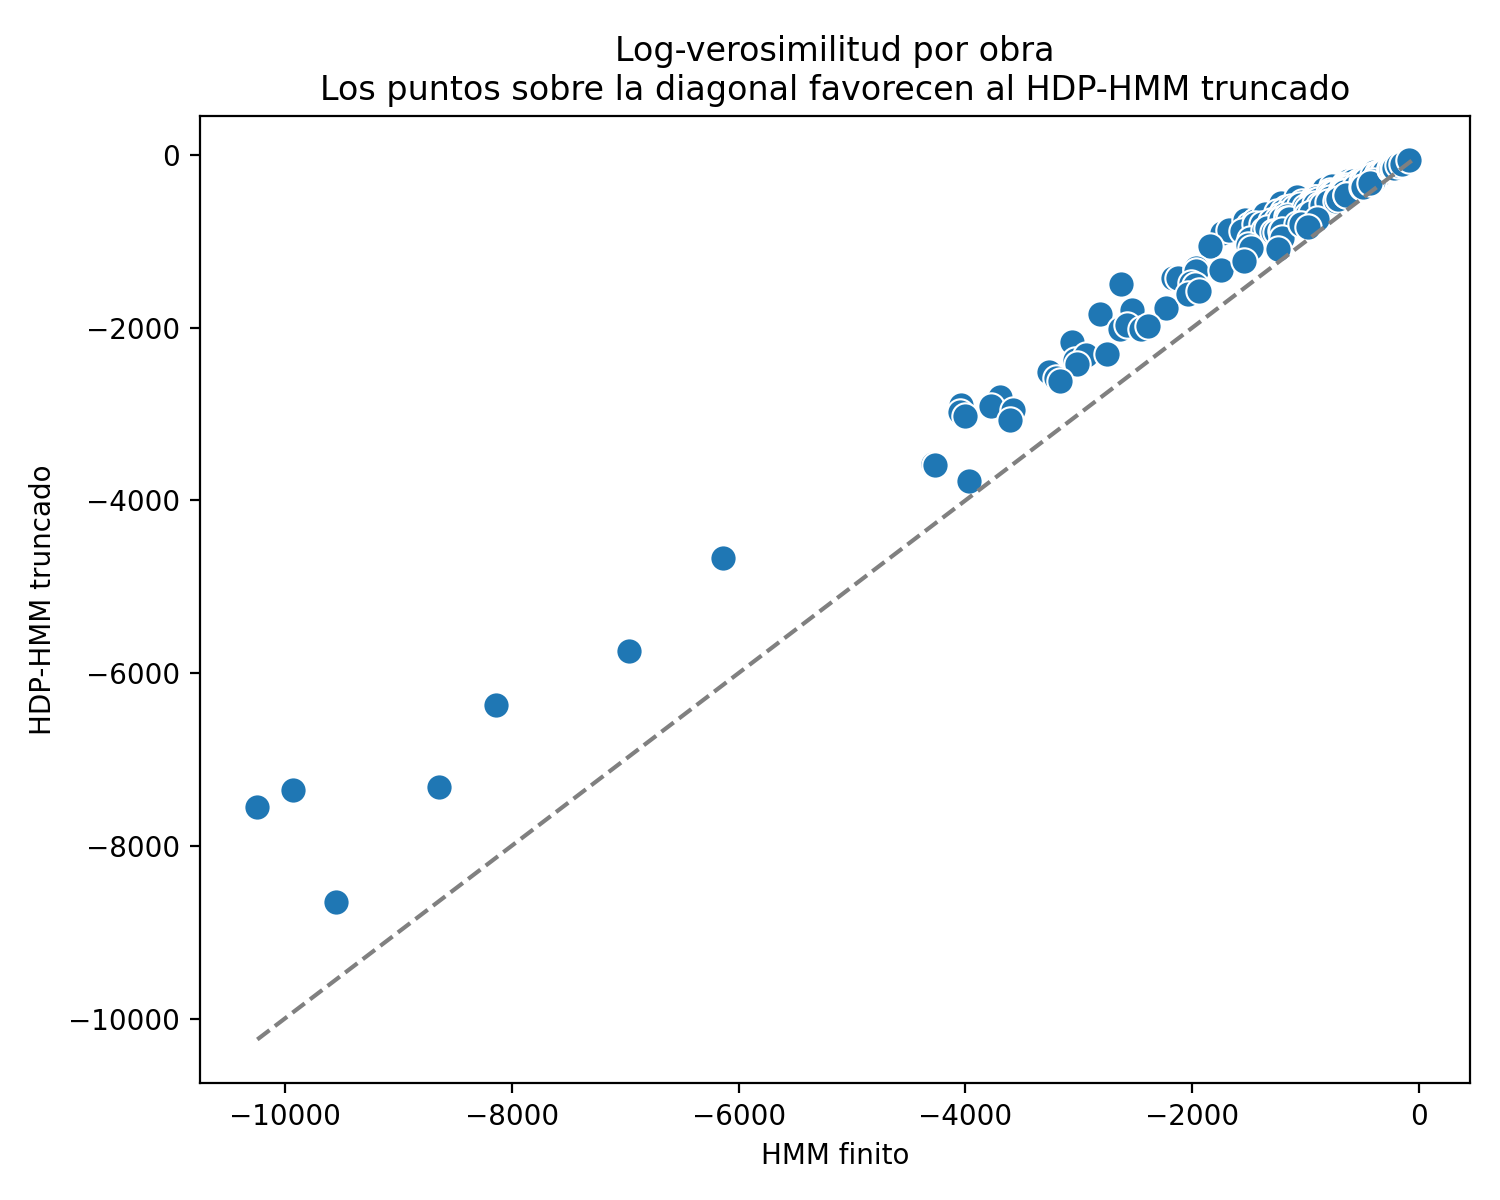
\includegraphics[width=\linewidth]{figures/chapter3/multicorpus_log_likelihood_scatter.png}
\caption{Comparación de log-verosimilitud por obra en el corpus extendido.}
\end{subfigure}

\medskip
\begin{subfigure}[t]{0.88\textwidth}
\centering
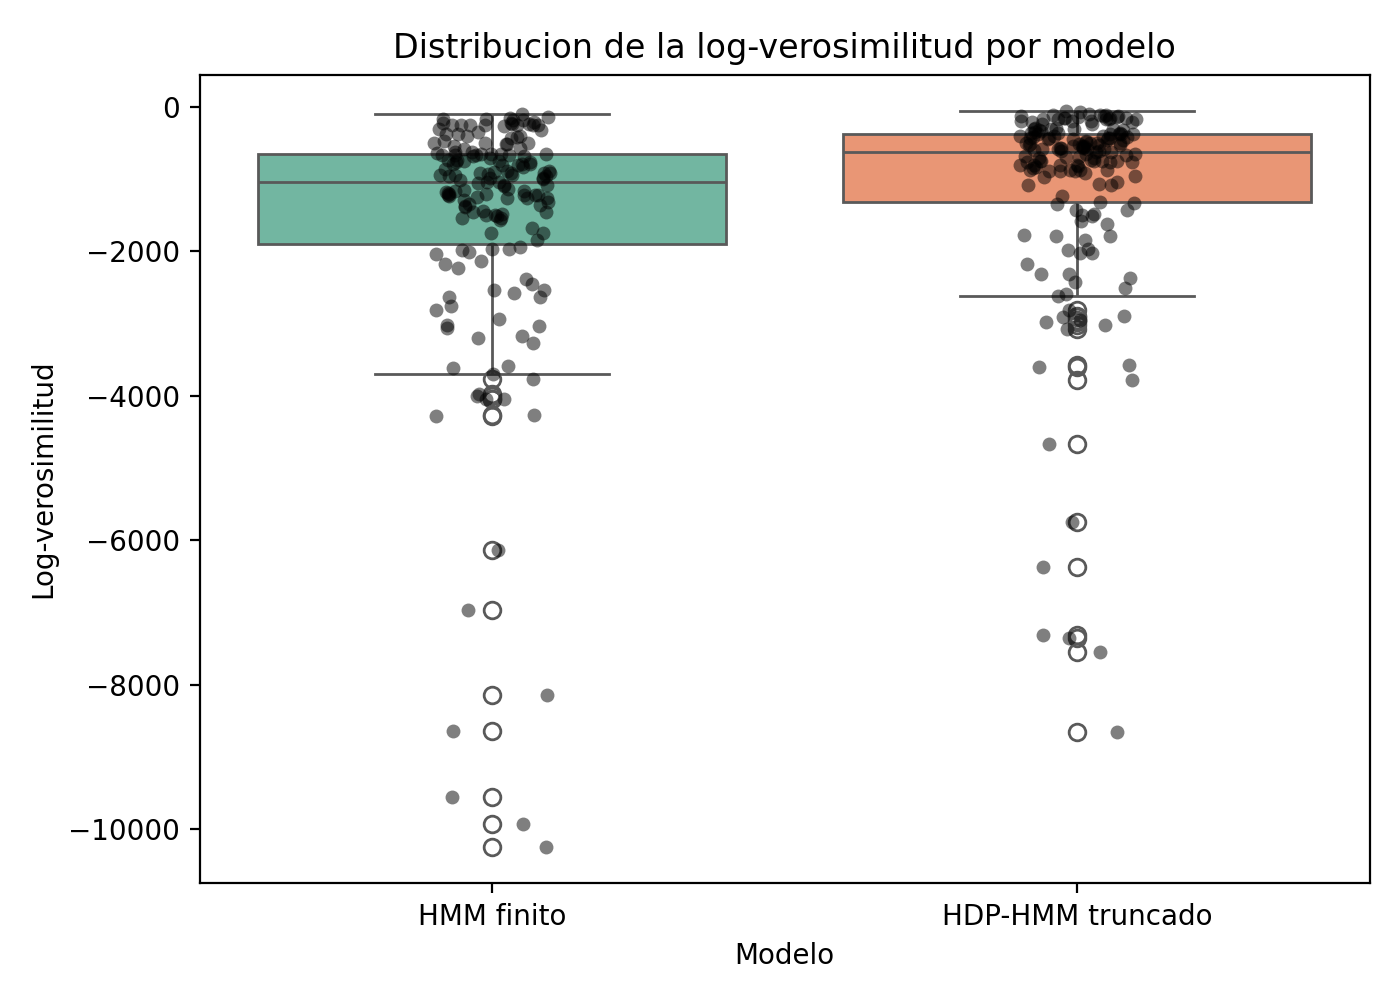
\includegraphics[width=\linewidth]{figures/chapter3/multicorpus_log_likelihood_boxplot.png}
\caption{Distribución agregada de log-verosimilitud por modelo.}
\end{subfigure}
\caption{Lectura visual del ajuste probabilístico sobre el corpus extendido. En ambos paneles, el desplazamiento favorece al HDP-HMM truncado.}
\label{fig:logverosimilitud-multicorpus}
\end{figure}

La Figura~\ref{fig:ganancia-y-complejidad-multicorpus} refuerza la misma lectura: la ganancia de log-verosimilitud es uniformemente positiva y el modelo truncado mantiene una ocupación efectiva de estados mucho más contenida que la del HMM finito.

\begin{figure}[H]
\centering
\begin{subfigure}[t]{0.88\textwidth}
\centering
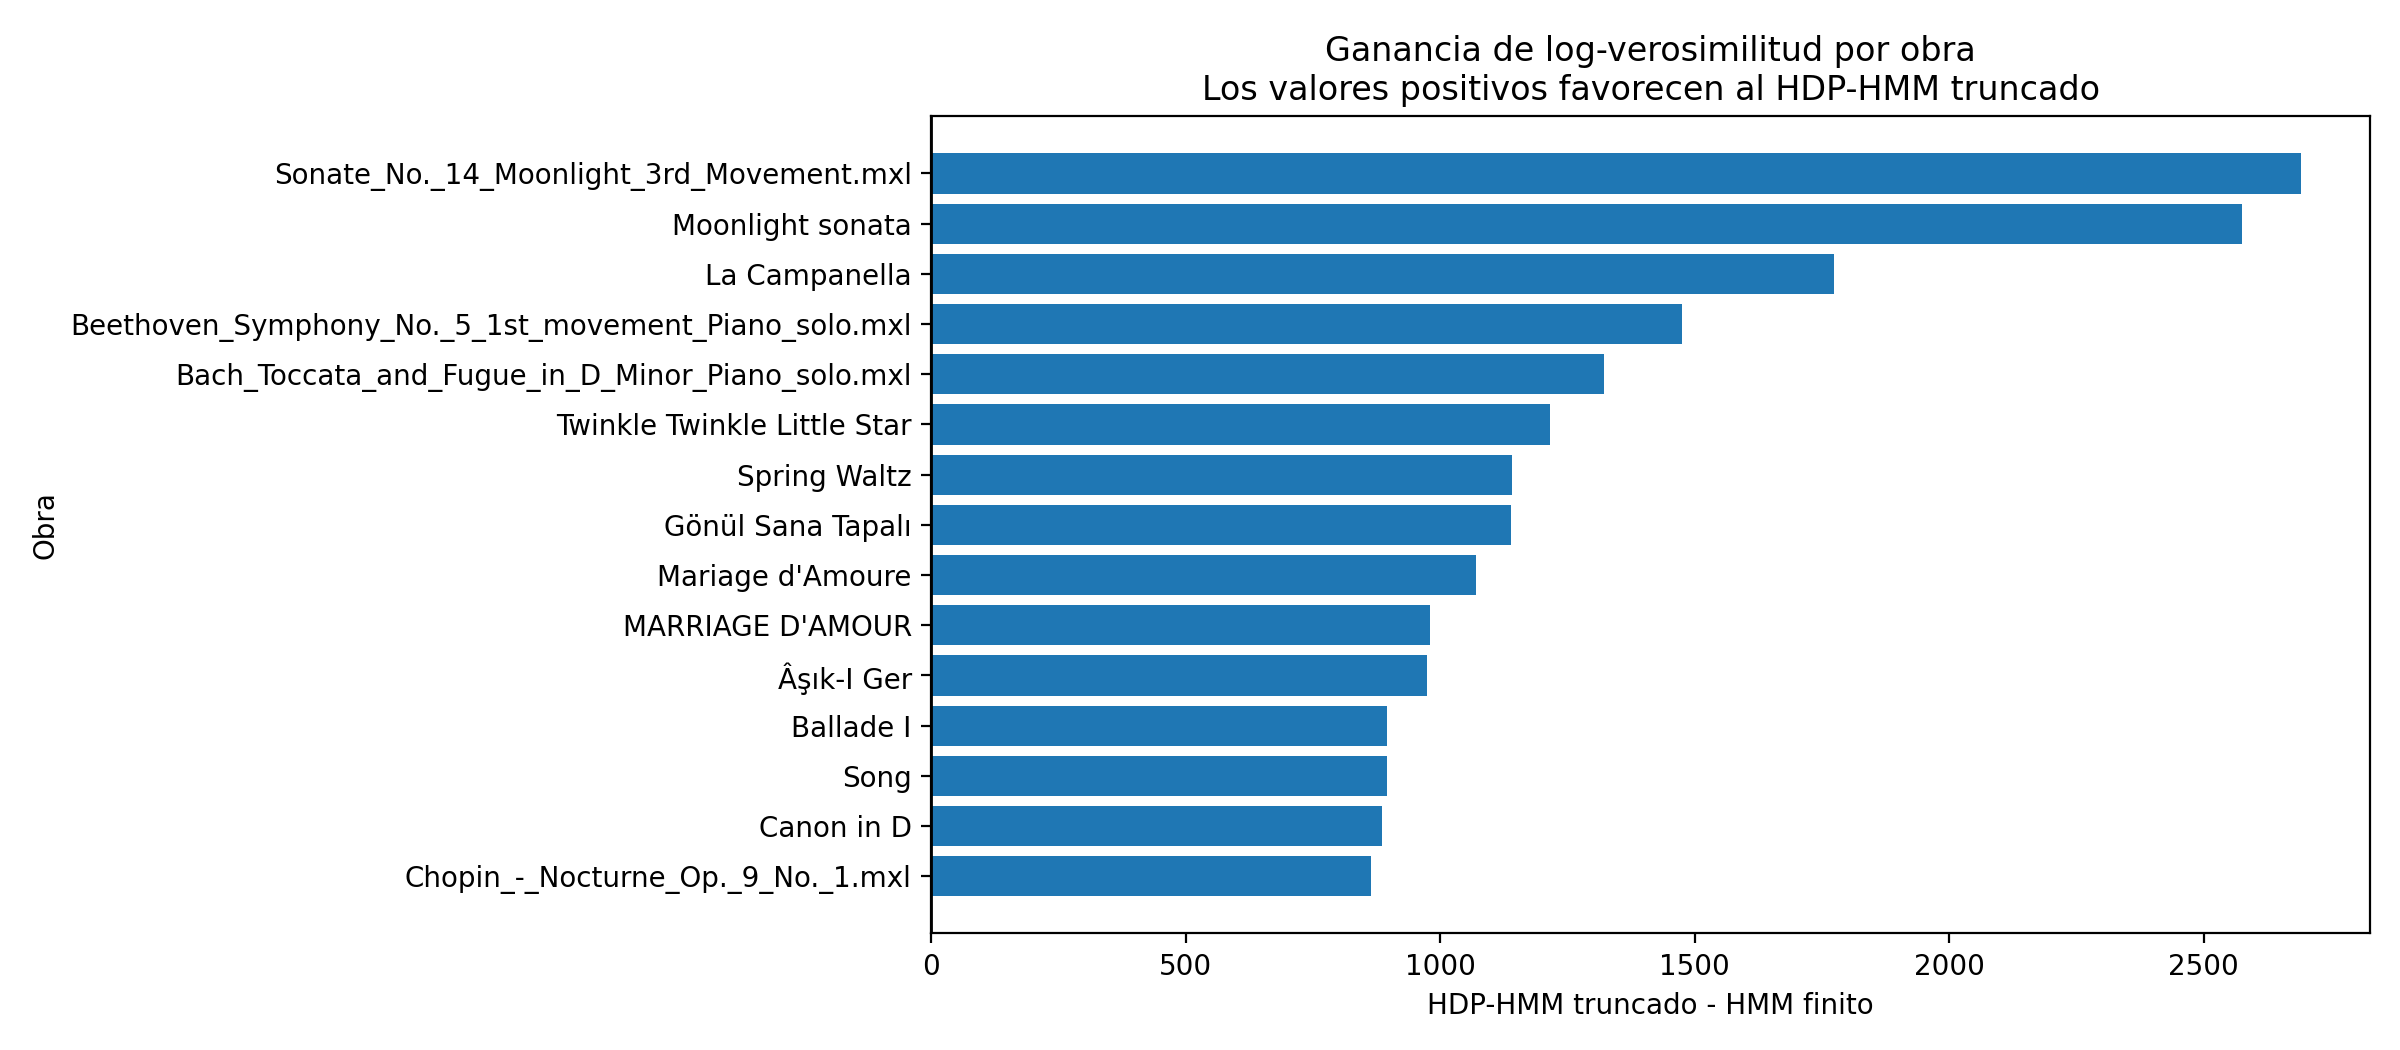
\includegraphics[width=\linewidth]{figures/chapter3/multicorpus_log_likelihood_gain_by_piece.png}
\caption{Ganancia de log-verosimilitud por obra.}
\end{subfigure}

\medskip
\begin{subfigure}[t]{0.88\textwidth}
\centering
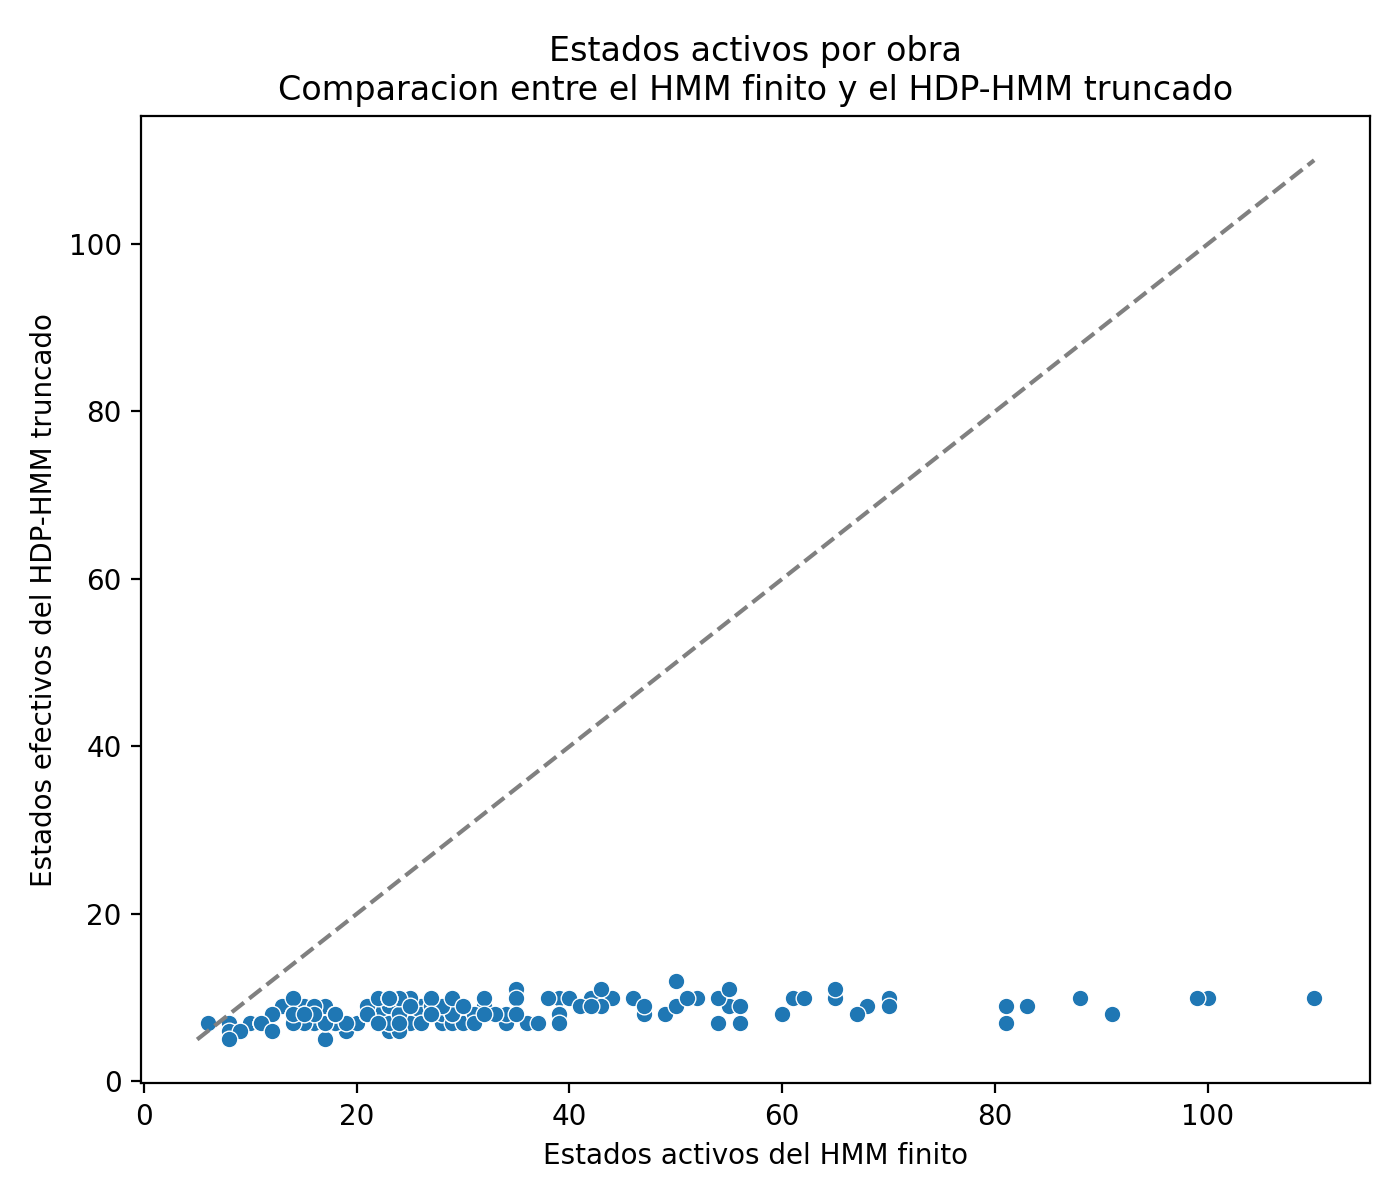
\includegraphics[width=\linewidth]{figures/chapter3/multicorpus_state_counts_scatter.png}
\caption{Comparación del número de estados utilizados por ambos modelos.}
\end{subfigure}
\caption{Ganancia y complejidad latente en el corpus extendido. El HDP-HMM truncado mejora el ajuste y, al mismo tiempo, mantiene una ocupación efectiva de estados mucho más contenida.}
\label{fig:ganancia-y-complejidad-multicorpus}
\end{figure}

La lectura crítica de esta evidencia exige distinguir entre mejora estadística y superioridad musicológica en sentido fuerte. En \texttt{SymbTr}, por ejemplo, la mejora no prueba que el vocabulario finito de referencia capture adecuadamente la teoría musical nativa del corpus; sí muestra, en cambio, que la aproximación truncada al modelo infinito es más robusta cuando el repertorio se vuelve heterogéneo. En conjunto, el corpus extendido fortalece la conclusión central del capítulo: truncar el iHMM no sólo vuelve viable la inferencia, sino que ofrece una realización empíricamente estable del principio no paramétrico, con mejor ajuste y complejidad efectiva menor.
